\chapter{Heuristics}\label{chap:heuristics}

\begin{quotation}
      \noindent ``It is not the strongest of the species that survives. It is also not the most intelligent that survives. It is the one that is the most adaptable to change.''
\end{quotation}
\begin{flushright}
      Charles Darwin
\end{flushright}

\noindent
Many different techniques have been used to train \acp{FFNN}~\cite{ref:kingma:2014}. Finding the best technique to use to train an \acs{FFNN} has been shown to be problem dependent in many cases~\cite{ref:kheiri:2017}. Every technique has its characteristics, constraints, advantages and disadvantages. At the time of writing, the majority of work that is published around the training of \acp{FFNN}, involves the use of gradient-based techniques~\cite{ref:nel:2021}. Gradient-based techniques are not without flaws and can, for example, yield slow convergence or get trapped in local optima~\cite{ref:mingguang:2009}. Other techniques have also been used to successfully train \acp{FFNN}, including meta-heuristics such as \acf{PSO}~\cite{ref:rakitianskaia:2012, ref:vanwyk:2014}, \acf{DE}~\cite{ref:espinal:2011} and \acfp{GA}~\cite{ref:gupta:1999}.

Chapter~\ref{chap:anns} briefly introduced the reader to the concept of \index{heuristic}\index{heuristic}heuristics and \index{meta-heuristic}meta-heuristics. This chapter presents more detailed background information on various different \index{heuristic}heuristics that have been used to train \acp{FFNN}. Broadly speaking, this chapter focuses on two different groups of \index{heuristic}heuristics, including classical gradient-based approaches and population-based \index{meta-heuristic}meta-heuristics. Each technique is presented and discussed in detail. Pseudo-code algorithms are provided for each technique and discussions follow on advantages, disadvantages, capabilities and limitations. The remainder of this chapter is structured as follows.

\begin{itemize}
      \item \textbf{Section~\ref{sec:heuristics:optimisation}} provides a brief review of optimisation. It is shown that training of \acp{FFNN} is an optimisation problem.

      \item \textbf{Section~\ref{sec:heuristics:what_is_a_heuristic}} provides background information on the origins and definition the term \index{heuristic}\textit{heuristic}. It is shown that \index{heuristic}heuristics are a class of algorithms that are used to solve optimisation problems.

      \item \textbf{Section~\ref{sec:heuristics:gd}} presents the reader with seven low-level, gradient-based \index{heuristic}heuristics, including \acf{SGD}, \acf{Momentum}, \acf{NAG}, \acf{Adagrad}, \acf{RMSProp}, \acf{Adadelta} and \acf{Adam}.

      \item \textbf{Section~\ref{sec:heuristics:mh}} presents the reader with three different population-baed \index{meta-heuristic}meta-heuristics, including \acf{PSO}, \acf{DE} and \acfp{GA}.

      \item \textbf{Section~\ref{sec:heuristics:summary}} provides the reader with a brief summary of the chapter.
\end{itemize}

\section{Optimisation}\label{sec:heuristics:optimisation}

Optimisation is the task of finding a solution to a given problem that is better than alternative solutions. Better stated by Oldewage~\cite{ref:oldewage:2017}, optimisation is the task of finding values for a set of variables such that some measure of optimality is satisfied given a set of constraints. Engelbrecht~\cite{ref:engelbrecht:2007} breaks optimisations problems down into three components:

\begin{itemize}
      \item An \textbf{objective function}: Represents the quantity to be optimised and is used as the ``measure of optimality''. Optimisation can be defined in terms of the minimisation or maximisation of the objective function $f$.

      \item A \textbf{set of unknowns or independent variables}: Affects the outcome of the objective function $f$ and is denoted as $x$. $f(x)$ is thus the quantification of the objective function over the unknowns, represented by $x$. Note that $x$ could be a scalar value, a vector or a matrix and notation is left out for simplicity.

      \item A \textbf{set of constraints}: Restrict and limit the values that can be assigned to the unknowns, represented by $x$. Optimisation problems that must adhere to a set of constraints are referred to as \acfp{CSP}.
\end{itemize}

\noindent
Optimisation problems come in a wide variety, and can be defined in terms of the number of variables used (uni- vs. multivariate), the number of objective functions used (single- vs. multi-objective), the degree of linearity (linear vs. quadratic/polynomial), the number of optima (uni- vs. multi-modal), the nature of the environment (static vs. dynamic), the types of variables used (separable vs. inseparable, discrete vs. continuous) and the set of constraints that the solution must adhere to (constrained vs unconstrained).

Optima can be defined as \textit{local} or \textit{global} optima. Local optima is the best optimisation of $f(x)$ in a neighbourhood of solutions, while the global optima is the best optimisation of $f(x)$ over all solutions in the solution space.

As stated in Chapter~\ref{chap:anns}, the training of an \acp{FFNN} is a particular type of optimisation problem, where the goal is to find the configuration of \textit{weights}, such that the \acs{FFNN} yields output that minimises some loss function. The mechanism by which the optimal weights for a \acs{FFNN} is sough out, is executed by an \index{optimisation algorithm}optimisation algorithm known as a \index{heuristic}heuristic. Discussions on the details of heuristics are presented in the following sections.

\section{What is a heuristic?}\label{sec:heuristics:what_is_a_heuristic}

The term \textit{heuristic} comes from the Latin word \textit{heuristicus} which means ``to find out or discover''.~\citeauthor{ref:romanycia:1985}~\cite{ref:romanycia:1985} provides a complete study on the history and origins of the term \index{heuristic}\textit{heuristic}. From their research, a proposal is made to define \index{heuristic}heuristics in the context of \acf{AI}, as any device, be it a program, rule, piece of knowledge, which is added to a problem-solving system, in expectation that on average, the performance will improve.

In the context of this dissertation, a \index{heuristic}heuristic refers to an algorithmic search technique that serves as a guide to a search process where good solutions to a optimisation problem is being sought out. Different \index{heuristic}heuristics make use of different information during the search process~\cite{ref:kheiri:2017}. During the training of \acp{FFNN}, \index{heuristic}heuristics such as gradient-based \index{heuristic}heuristics make use of the derivatives obtained by evaluating the \acs{FFNN}. It can thus be said that gradient-based \index{heuristic}heuristics make use of information directly from the \textit{search space}. On the contrary, \index{heuristic}heuristics such as \index{hmeta-euristic}meta-heuristics make use of meta-information obtained as a result of evaluating the \acs{FFNN}~\cite{ref:blum:2003}. The meta-information that \index{meta-heuristic}meta-heuristics make use of could include ranked-performance of a population of candidate solutions, referred to as \textit{entities}. \index{meta-heuristic}Meta-heuristics are useful when there is imperfect information about the search space~\cite{ref:bianchi:2009}, and are generally less problem-specific than other classes of \index{heuristic}heuristics~\cite{ref:blum:2003}. This disseration takes a particular interest in gradient-based \index{heuristic}heuristics and \index{meta-heuristic}meta-heuristics. Each of these are presented in detail in the following sections.


\section{Gradient-Based Heuristics}\label{sec:heuristics:gd}

Gradient-based \index{heuristic}heuristics are optimisation techniques that make use of derivates obtained from evaluating the model being optimised. Specifically, in the context of a minimisation problem, these techniques are called \acf{GD} heuristics as they \textit{minimise} some loss function. \Acs{GD} is generally attributed to Cauchy~\cite{ref:lemarechal:2012}, who first suggested it in 1847. In 1907 Hadamard~\cite{ref:hadamard:1908} independently proposed a similar method.

Although \acs{GD} \index{heuristic}heuristics where not the first \index{heuristic}heuristics used to train \acp{FFNN}
\cite{ref:engelbrecht:2007}, they are certainly the most whidely used. \Acs{GD} heuristics have become increasingly popular partly due to their simplicity and low computational overhead compared to other \index{heuristic}heuristics such as \index{meta-heuristic}meta-heuristics and other second-order derivative methods such as Newtons' method. There are many variants of \acs{GD} \index{heuristic}heuristics, however, they all fundamentally apply the same generic \acs{GD} framework called \acl{BP}.

\subsection{Backpropagation}\label{sec:heuristics:gd:backpropagation}

Chapter~\ref{chap:anns} introduced the reader to \index {supervised learning}supervised learning and presented a number of loss functions. In the context of supervised learning, loss functions produce a scalar value $\epsilon$, that represents the error between the output of the \acs{FFNN} and the desired output. When using \acs{GD} to train \acp{FFNN}, the \index{loss function}loss function is used to adjust the weights of the \acs{FFNN} in order to minimise the error~\cite{ref:engelbrecht:2007}.~\citeauthor{ref:engelbrecht:2007}~\cite{ref:engelbrecht:2007} states that training of \acp{FFNN} using \acs{GD}, is done by calculating the gradient of $\epsilon$ in \textit{weight-space}, and then moving the weight vector along the negative gradient. An illustration of \acs{GD} is given in Figure~\ref{fig:heuristics:gd:gd_illustration}.

\begin{figure}[htbp]
      \centering
      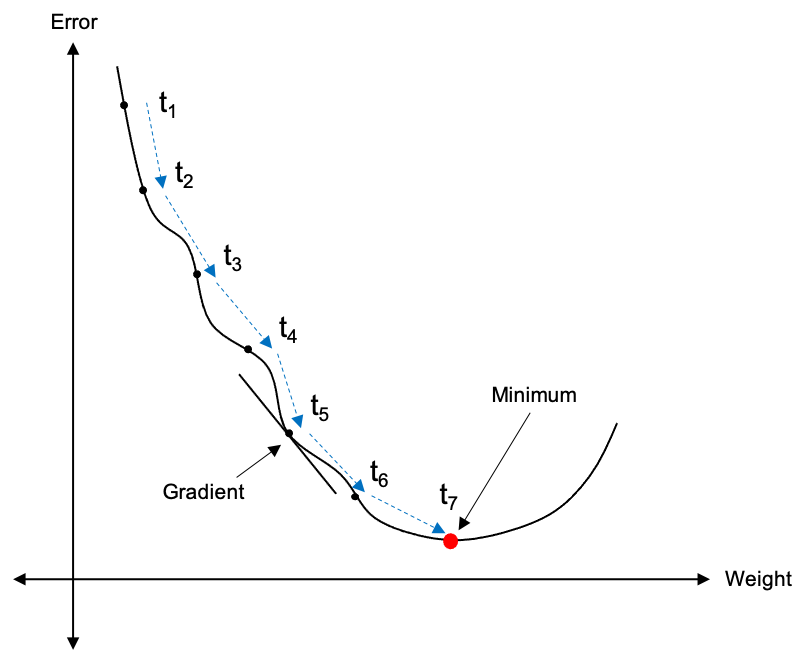
\includegraphics[width=0.85\textwidth]{images/gradient_descent.pdf}
      \caption{An illustration of \acs{GD} over various timesteps showing the minimisation of the error with regards to weight value.}
      \label{fig:heuristics:gd:gd_illustration}
\end{figure}

\noindent
The update step for \acs{GD} can be formulated as is shown in Equation~\eqref{eq:heuristics:gd:update_step_part_1} below.

\begin{equation}
      \label{eq:heuristics:gd:update_step_part_1}
      w_{i}(t) = w_{i}(t-1) + \Delta w_{i}(t)
\end{equation}

\noindent
In Equation~\eqref{eq:heuristics:gd:update_step_part_1} above, the delta weight $\Delta w$, at index $i$ and timestep $t$ is given by Equation~\eqref{eq:heuristics:gd:update_step_part_2} below.

\begin{equation}
      \label{eq:heuristics:gd:update_step_part_2}
      \Delta w_{i}(t) = -\eta\frac{\partial \epsilon}{\partial w_{i}}
\end{equation}

\noindent
In Equation~\eqref{eq:heuristics:gd:update_step_part_2} above, $\eta$ is the learning rate. The learning rate is an important hyper-parameter in gradient-based \index{heuristic}heuristic as it controls the step-size that is taken in the direction of the negative gradient at each timestep. Assuming the use of \acs{SSE} as the loss function, the partial derivative of $\epsilon$, relative to the weight $w$, at index $i$, is given by Equation~\eqref{eq:heuristics:gd:update_step_part_3} below.

\begin{equation}
      \label{eq:heuristics:gd:update_step_part_3}
      \frac{\partial \epsilon}{\partial w_{i}} = -2(t_{p} - o_{p})\frac{\partial f}{\partial net_{p}}z_{i,p}
\end{equation}

\noindent
In the context of training \textit{shallow} \acp{FFNN} using \index{supervised learning}supervised learning, the error signal is propagated backwards in the network from the output layer, through the hidden layer. The algorithm that propagates the error signal backwardds is known as \acf{BP}. \Acs{BP} was popularised by~\citeauthor{ref:werbos:1994}~\cite{ref:werbos:1994}.~\citeauthor{ref:nel:2021}~\cite{ref:nel:2021} states that \acs{BP} provides a procedure for updating the network weights, layer by layer, by evaluating the derivatives of the error function $\epsilon$ with respect to the weights at each layer.~\citeauthor{ref:engelbrecht:2007}~\cite{ref:engelbrecht:2007}describes the \acs{BP} process in two steps:

\begin{itemize}
      \item \textbf{Feedforward Pass}: During this phase the output values of the \acs{FFNN} is calculcated for each training pattern.
      \item \textbf{Backward Propagation}: During this phase the error signal that is calculated as is shown above in Equations~\eqref{eq:heuristics:gd:update_step_part_1}-~\eqref{eq:heuristics:gd:update_step_part_3} is propagated backwards from the output layer, through the hidden layer, to the input layer of the \acs{FFNN}. Weights are then adjusted as functions of the backpropagated error signal.
\end{itemize}


\subsection{Stochastic Gradient Descent}\label{sec:heuristics:gd:sgd}

This section shines light on the algorithmic implementation of \ac{BP} with specific context to \ac{SGD}. The algorithm is provided followed by a simplification of the update-step that provides the basis for the next gradient-based heuristics that follow.

The pseudo-code implementation for the \acs{SGD} algorithm is taken from~\cite{ref:engelbrecht:2007} and is presented in Algorithm~\ref{algo:heuristics:gd:sgd} below.

\begin{algorithm}[H]
      \caption{The pseudo code algorithm for the \acs{SGD} heuristic.}
      \label{algo:heuristics:gd:sgd}
      \begin{algorithmic}
            \State Initialise weights, $\eta$, $\alpha$ and the number of epochs $t=0$;
            \While{stopping condition not met}
            let $\epsilon_{T} = 0$
            \For{each training pattern p}
            \State Do the feedforward pass phase to calculate $y_{j,p}$ ($\forall j = 1, \dots, J$) and $o_{k,p}$ ($\forall k = 1, \dots, K$);
            \State Compute the output error signals $\delta_{o_{k,p}}$ and the hidden layer error signals $\delta_{y_{j,p}}$;
            \State Adjust the weights $w_{kj}$ and $v_{ji}$ (backpropagation of errors);
            \State $\epsilon_{T}$ += $[\epsilon_{p} = \sum^{K}_{k=1}(t_{k,p} - o_{k,p})^{2}]$;
            \EndFor
            \State $t = t + 1$;
            \EndWhile
      \end{algorithmic}
\end{algorithm}

In order to provide a simplified frame of reference from which the gradient-based heuristics are compared, consider a simplification of the update-step for the weights of the \acs{FFNN} as is done using \ac{SGD} below.

\begin{equation}
      \label{eq:heuristics:gd:sgd}
      \begin{split}
            w = w - \eta \nabla_{w}\mathcal{E}(w)
      \end{split}
\end{equation}

In Equation~\ref{eq:heuristics:gd:sgd} $w$ refers to the weights of the \acs{FFNN}, $\eta$ refers to the learning rate as before and $\nabla_{w}\mathcal{E}(w)$ refers to the gradient of the loss/cost function w.r.t the output of the \acs{FFNN} as a result of its weights. Note that all subscripts w.r.t. layers and training patterns are omitted for convenience.

So far detailed mathematical descriptions have been provided to illustrate the concept of \ac{GD} and how it applies to the \acs{SGD} heuristic as applied to \ac{FFNN} training. It was mentioned that \ac{SGD} was one of the first widely used heuristics to train \ac{FFNN}, however, it is not without flaws. With stochastic learning, only one training pattern is presented at each iteration. As such, weight updates are done with high variance and noise~\cite{ref:ruder:2016}. An illustration of the the fluctuations caused by \ac{SGD} during training is given in Figure~\ref{fig:heuristics:gd:sgd}.

\begin{figure}[htbp]
      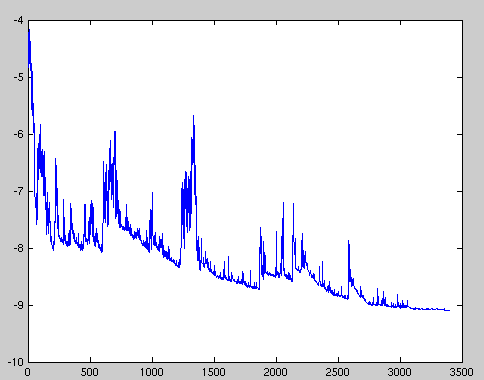
\includegraphics[width=\textwidth]{images/sgd.png}
      \caption{An illustration of \ac{SGD} fluctuations during training as taken from~\cite{ref:sgd:2006}.}
      \label{fig:heuristics:gd:sgd}
\end{figure}

With batch learning, all the training patterns are presented at once and the \acs{FFNN} converges to the minimum of the loss/cost function w.r.t $w$. However, this is computationally expensive and intractable to implement in many situations. While \ac{SGD} is able to jump out of local minima into new, potentially better local minima~\cite{ref:ruder:2016}, it does at first this seems advantageous. However, this complicates convergence to the exact minima as \ac{SGD} can potentially keep overshooting better minima. It is shown that a slow decrease in the learning rate $\eta$ will lead to the same convergence behaviour as with batch learning, almost certainly converging to local or global minima for non-convex and convex optimisation respectively. A compromise to this problem is to include mini-batches of training patterns where a small number of training patterns are presented to the \acs{FFNN} at once. This means that the input patterns from mini-batches are just approximations of the total population of training patterns. According to~\citeauthor{ref:ruder:2016}~\cite{ref:ruder:2016} this has two main advantages

\begin{itemize}
      \item Reduces the high variance of weight updates which leads to better convergence
      \item Allows for the implementation of \ac{SGD} using highly optimised matrix operations, common to the state-of-the-art \ac{ML} libraries used today.
\end{itemize}

In the context of this dissertation, \ac{SGD} refers to the mini-batch learning implementation. Although mini-batch \ac{SGD} does provide a compromise between single-pattern and batch learning there are still a number of challenges posed by this approach. These include:

\begin{itemize}
      \item The appropriate value to use for the learning rate $\eta$ is difficult to determine and is often problem-specific. A learning rate that is too small causes premature exploitation, leading to slow and bad convergence. On the contrary, a learning rate that is too high may lead to bad learning outcomes as the heuristic keeps overshooting good minima.

      \item Learning rate schedules~\cite{ref:robbins:1951} can be introduced to dynamically change the learning rate throughout the training process, however, these schedules and their parameters have to be defined a priori and are thus problem specific~\cite{ref:darken:1992}.

      \item The learning rate that has been introduced so far is applied to all weight updates. If the training data is sparse and the features have very different frequencies an equal update to all weights is inefficient. Larger weight updates are required for less frequently occurring features. This problem eludes to the credit assignment problem~\cite{ref:rumelhart:1986} common to these \ac{GD} variants.

      \item It is difficult to avoid getting trapped in local minima, especially for highly non-convex loss/cost functions used for \ac{ANN} training.~\cite{ref:dauphin:2014} argues that this difficulty arises not from local minima, but from sadle points. Sadle points are points at which one dimensions slopes upwards while another dimension slopes downwards.~\cite{ref:ruder:2016} mentions that these sadle points are usually surrounded by plateaus of the same error, leading to gradients that are close to zero in all dimensions.
\end{itemize}


Alternative methods have been proposed that lead to better control over the convergence characteristics caused by \ac{GD} variants. The first of these include \ac{Momentum} and is presented next.


\subsection{Momentum}
\label{sec:heuristics:gd:momentum}

Research shows that \ac{SGD} has difficulty navigating ravines i.e. areas where the surface curves much more steeply in one dimension than in another~\cite{ref:sutton:1986}. These ravines are common around local minima. As such, \ac{SGD} is shown to oscillate across the slopes of the ravine while only making minor progress towards the local minima. An illustration of this is given in Figure~\ref{fig:heuristics:gd:sgd_with_and_without_momentum}.

\begin{figure}[htbp]
      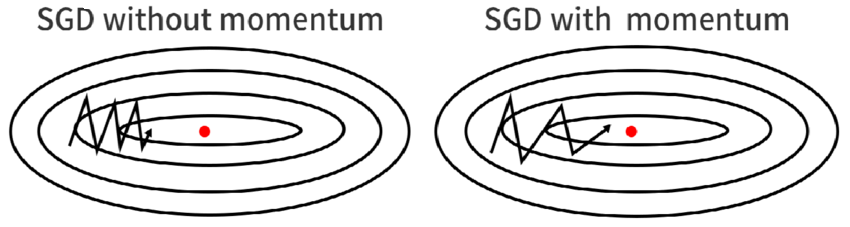
\includegraphics[width=\textwidth]{images/sgd_with_and_without_momentum.png}
      \caption{An illustration of \ac{SGD} with and without momentum taken from~\cite{ref:du:2019}.}
      \label{fig:heuristics:gd:sgd_with_and_without_momentum}
\end{figure}

Momentum~\cite{ref:qian:1999} is a variant of the \acs{SGD} that helps accelerate \ac{SGD} in the relevant direction, dampening oscillations.~\cite{ref:ruder:2016} mentions that this is done by adding a fraction $\alpha$ of the weight update vector of the previous timestep to the current weight update vector. The accumulation of momentum is presented in Equation~\ref{eq:heuristics:gd:momentum_part_1} while the update step is then amended in Equation~\ref{eq:heuristics:gd:momentum_part_2} below.

\begin{equation}
      \label{eq:heuristics:gd:momentum_part_1}
      \begin{split}
            v_{t} = \alpha v_{t-1} + \eta \nabla_{w}\mathcal{E}(w)
      \end{split}
\end{equation}

\begin{equation}
      \label{eq:heuristics:gd:momentum_part_2}
      \begin{split}
            w = w - v_{t}
      \end{split}
\end{equation}

By redefining the \acs{SGD} update steps as shown above, the \acs{Momentum} heuristic allows for the increase of momentum for dimensions whose gradients point in the same direction, while simultaneously reducing momentum for dimensions whose gradients change direction, leading to faster convergence and less oscillation. The momentum term $\alpha$ is usually set to 0.9~\cite{ref:engelbrecht:2007}\cite{ref:ruder:2016}.


\subsection{Nesterov Accelerated Gradients}
\label{sec:heuristics:nag}

\Acl{NAG} is a variant of the \acs{Momentum} heuristics developed by Ilya Sutskever~\cite{ref:sutskever:2013-2} and is inspired from Yurii Nesterov's~\cite{ref:nesterov:1983} work on optimising convex functions. \ac{NAG} provides an improvement to the momentum accumulation term by providing a look-ahead term that better refines the weight update step. In the \acs{NAG} heuristic, the gradient is not calculated w.r.t the current weights, but rather w.r.t the approximate future positions of the weights~\cite{ref:ruder:2016}. An illustration of this is taken from Geoffrey Hinton's lecture on mini-batch \ac{GD}~\cite{ref:hinton:2012} and is presented in Figure~\ref{fig:heuristics:gd:nag} below.

\begin{figure}[htbp]
      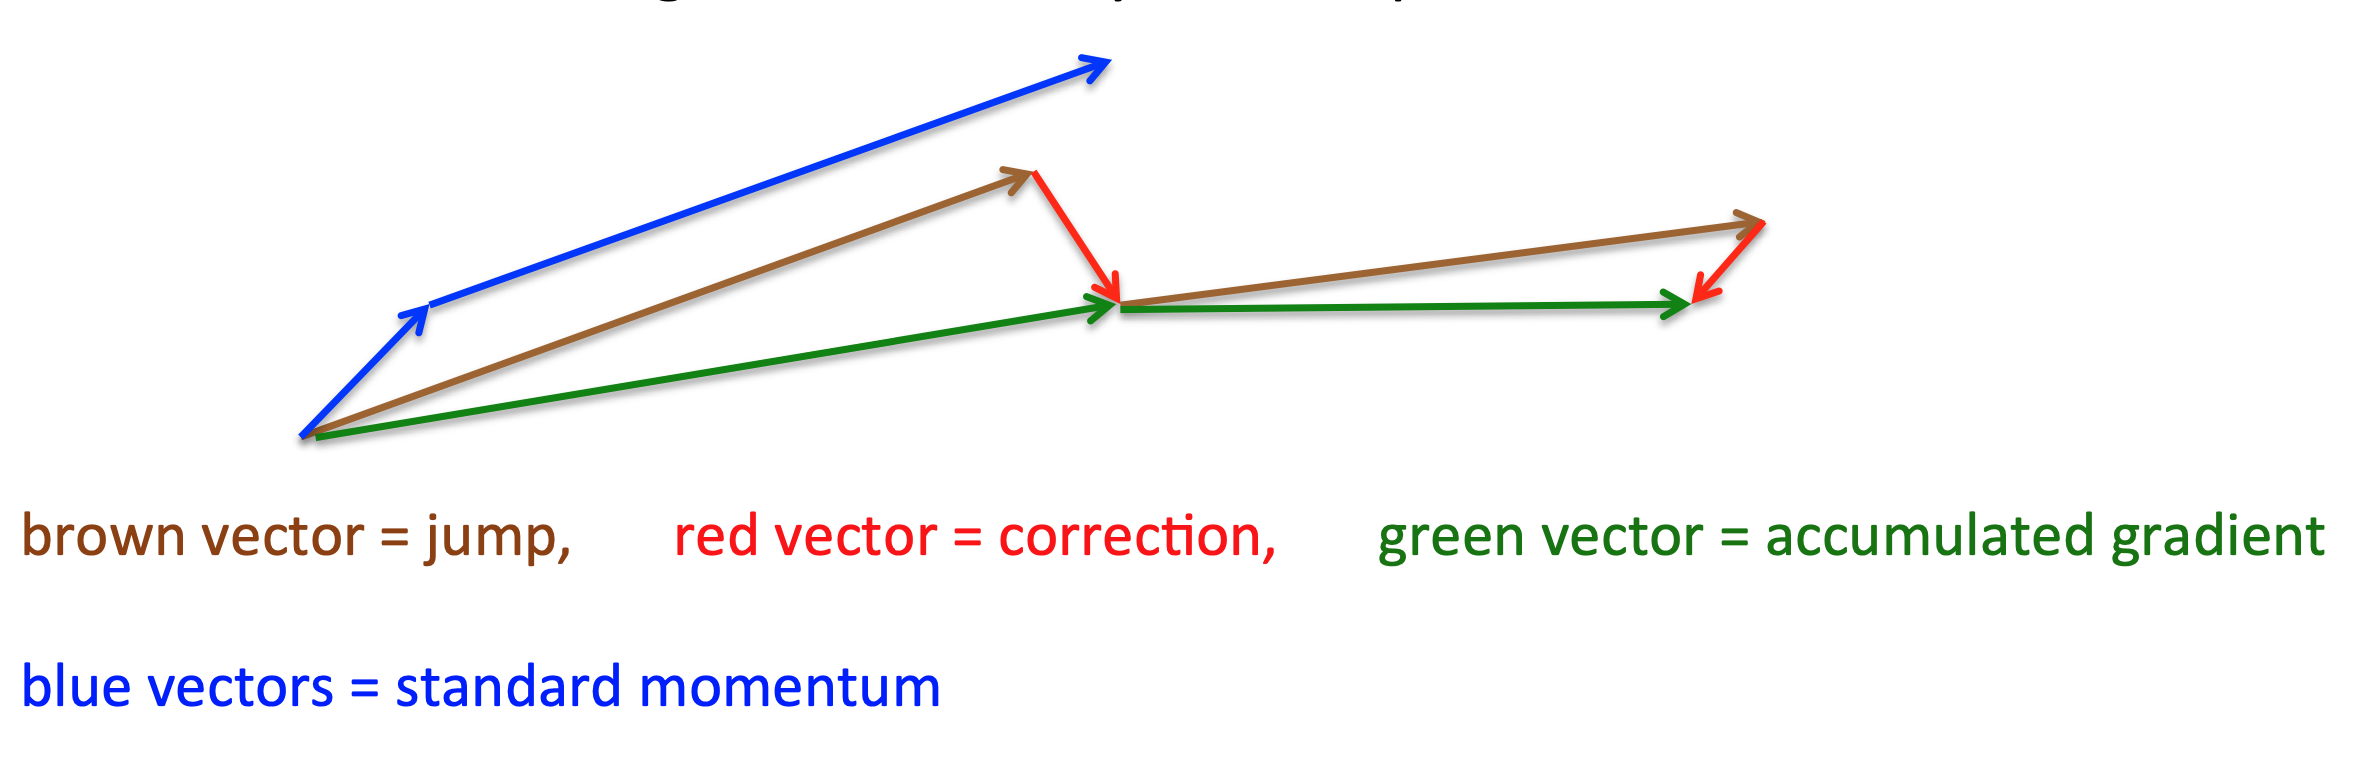
\includegraphics[width=\textwidth]{images/nag.png}
      \caption{An illustration of the weight update vector for \ac{NAG} taken from~\cite{ref:hinton:2012}.}
      \label{fig:heuristics:gd:nag}
\end{figure}


\citeauthor{ref:ruder:2016}~\cite{ref:ruder:2016} explains the update step as is done by \ac{NAG} is follows. \ac{Momentum} first computes the current gradient. This is seen by the small blue vector presented in Figure~\ref{fig:heuristics:gd:nag}. A large step is taken in the direction of the updated accumulated gradient, presented by the big blue vector. \ac{NAG} then first takes a big step in the direction of the previous accumulated gradient presented by the brown vector. At this point the gradient is measured and \ac{NAG} then makes a correction (red vector), which results in the complete NAG update (green vector). By anticipating approximate future positions of the weights, the weight update step as defined by \ac{NAG} controls the optimisation process from from going too fast and results in increased responsiveness. The \ac{NAG} weight vector update steps are given in Equations~\ref{eq:heuristics:gd:nag_part_1} and~\ref{eq:heuristics:gd:nag_part_2} below.

\begin{equation}
      \label{eq:heuristics:gd:nag_part_1}
      \begin{split}
            v_{t} = \alpha v_{t-1} + \eta \nabla_{w}\mathcal{E}(w - \alpha v_{t-1})
      \end{split}
\end{equation}

\begin{equation}
      \label{eq:heuristics:gd:nag_part_2}
      \begin{split}
            w = w - v_{t}
      \end{split}
\end{equation}

The next logical step in the improvement of the weight vector update step is to tailor the update steps for each weight parameter controlling the magnitude of the update step based on the relevance and importance for that dimension.

\subsection{Adaptive Gradients}
\label{sec:heuristics:adagrad}

\Acl{Adagrad} is an adaptation of \ac{SGD} which implements a learning rate for every parameter in the weight vector and is developed by Duchi et al.~\cite{ref:duchi:2011}.~\citeauthor{ref:ruder:2016}~\cite{ref:ruder:2016} mentions that \Ac{Adagrad} adapts the learning rate to the weights, performing small updates (i.e. low learning rates) for weights associated with frequently occurring features and larger updates (i.e. high learning rates) for weights associated with infrequent features. For this reason \ac{Adagrad} is well suited for dealing with situations with very sparse training data.

In the \acs{GD} variants presented thus far, the weight updates have been applied to all weights at once using the same learning rate $\eta$ for all dimensions of the weight update vector. \Ac{Adagrad} uses a different learning rate for every weight $w_{i}$ at every timestep $t$. The weight update step as implemented by \ac{Adagrad} is presented in Equation~\ref{eq:heuristics:gd:adagrad_part_1} below.

\begin{equation}
      \label{eq:heuristics:gd:adagrad_part_1}
      \begin{split}
            w_{t+1,i} = w_{t,i} - \frac{\eta}{\sqrt{G_{t,ii} + \epsilon}}.\nabla_{w_{i}}\mathcal{E}(w_{t,i})
      \end{split}
\end{equation}

where $w_{i}$ is the $i$-th dimension of the weight vector, $G_{ii} \in \mathbb{R}^{d \times d}$ is a diagonal matrix where each diagonal element $i,i$ is the sum of the squared of the gradients w.r.t. $w_{i}$ up to timestep $t$ and $\epsilon$ is a smoothing term that avoids division by zero, usually set in the order of $1 \times 10^{-8}$~\cite{ref:ruder:2016}. Since $G_{t}$ contains the sum of the squares of the gradients with respect to all parameters $w$ along its diagonal, the weight update step can be vectorised and updated using the matrix-vector product between $G_{t}$ and $\nabla_{w_{i}}\mathcal{E}(w_{i})$. This is presented in Equation~\ref{eq:heuristics:gd:adagrad_part_2} below.

\begin{equation}
      \label{eq:heuristics:gd:adagrad_part_2}
      \begin{split}
            w_{t+1} = w_{t} - \frac{\eta}{\sqrt{G_{t} + \epsilon}} \odot \nabla_{w_{i}}\mathcal{E}(w_{t})
      \end{split}
\end{equation}

\Ac{Adagrad}'s main benefit is that it does not require the need to manually tune the learning rate. However, a problem with \ac{Adagrad} is the accumulation of the sums of squared gradients in the denominator. Since every term that is added is positive, this number keeps growing, leading to a situation where the learning rate shrinks to the point that the heuristic is no longer able to learn. \acl{Adadelta} aims to improve on this problem.

\subsection{Adaptive Learning Rate}
\label{sec:heuristics:adadelta}

In Section~\ref{sec:heuristics:adagrad} it was mentioned that one of the main problems of \ac{Adagrad} is that it has an aggressively monotonically decreasing learning rate because of the accumulation of the sum of squared gradients in its denominator. Zeiler~\cite{ref:zeiler:2012} presents an improvement on \ac{Adagrad} that eliminates this problem.~\citeauthor{ref:ruder:2016}~\cite{ref:ruder:2016} mentions that instead of accumulating all past squared gradients as in the case of \ac{Adagrad}, \ac{Adadelta} restricts the window of accumulation to a window with a fixed size $W$. However, storing $W$ previous squared gradients is very inefficient. Instead, the accumulation of the sum of gradients over $W$ steps is defined recursively as a decaying average of all past squared gradients. The moving average $E[g^{2}]_{t}$ at timestep $t$ then depends only a fraction $\alpha$ of the previous average and current gradient, similar to the update step for \ac{Momentum}. In order to simplify the notation of update steps, let $g = \nabla_{w_{i}}\mathcal{E}(w_{t})$. The moving average update step for $E[g^{2}]_{t}$ is then presented in Equation~\ref{eq:heuristics:gd:adadelta_part_1} below.

\begin{equation}
      \label{eq:heuristics:gd:adadelta_part_1}
      \begin{split}
            E[g^{2}]_{t} = \alpha E[g^{2}]_{t - 1} + (1 - \alpha)g_{t}^{2}
      \end{split}
\end{equation}

The value for $\alpha$ is set to a similar value, 0.9, as was done with \ac{Momentum}. For sake of clarity, the basic \ac{SGD} update step is rewritten in terms of the weight update vector $\Delta w_{t}$. This is presented in Equations~\ref{eq:heuristics:gd:adadelta_part_2} and~\ref{eq:heuristics:gd:adadelta_part_2} below.

\begin{equation}
      \label{eq:heuristics:gd:adadelta_part_2}
      \begin{split}
            \Delta w_{t} = -\eta g_{t,i}
      \end{split}
\end{equation}

\begin{equation}
      \label{eq:heuristics:gd:adadelta_part_3}
      \begin{split}
            w_{t+1} = w_{t} + \Delta w_{t}
      \end{split}
\end{equation}

The weight update vector for \ac{Adagrad} as defined in Equation~\ref{eq:heuristics:gd:adagrad_part_2} is then rewritten as


\begin{equation}
      \label{eq:heuristics:gd:adagrad_part_2_new}
      \begin{split}
            \Delta w_{t} = - \frac{\eta}{\sqrt{G_{t} + \epsilon}} \odot g_{t}
      \end{split}
\end{equation}

The diagonal matrix $G_{t}$ is then replaced with the decaying average over the past $W$ squared gradients as presented in Equation~\ref{eq:heuristics:gd:adadelta_part_4} below.

\begin{equation}
      \label{eq:heuristics:gd:adadelta_part_4}
      \begin{split}
            \Delta w_{t} = - \frac{\eta}{\sqrt{E[g^{2}]_{t} + \epsilon}} g_{t}
      \end{split}
\end{equation}

Since the denominator is the \acs{RMS} error criterion of the gradient, the criteria short-hand notation is used as follows.

\begin{equation}
      \label{eq:heuristics:gd:adadelta_part_5}
      \begin{split}
            \Delta w_{t} = - \frac{\eta}{RMS[g]_{t}} g_{t}
      \end{split}
\end{equation}

\citeauthor{ref:ruder:2016}\cite{ref:ruder:2016} highlights that the original authors~\cite{ref:zeiler:2012} noted that the units of the update step as presented in Equation~\ref{eq:heuristics:gd:adadelta_part_2} do not match i.e. the update vector should have the same hypothetical units as the weight vector. To realize this, another exponentially decaying average is defined in terms of squared weight updates as is presented in Equation~\ref{eq:heuristics:gd:adadelta_part_6} below.

\begin{equation}
      \label{eq:heuristics:gd:adadelta_part_6}
      \begin{split}
            E[\Delta w^{2}]_{t} = \alpha E[\Delta w^{2}]_{t - 1} + (1 - \alpha)\Delta w^{2}
      \end{split}
\end{equation}

The \ac{RMS} error of weight updates is thus

\begin{equation}
      \label{eq:heuristics:gd:adadelta_part_7}
      \begin{split}
            RMS[\Delta w]_{t} = \sqrt{E[\Delta w^{2}]_{t} + \epsilon}
      \end{split}
\end{equation}

Note that $RMS[\Delta w]_{t}$ is unknown at timestep $t$. It is thus approximated with the \acs{RMS} of weight updates until the previous timestep. The learning rate in Equation~\ref{eq:heuristics:gd:adadelta_part_5} is then replaced as follows.

\begin{equation}
      \label{eq:heuristics:gd:adadelta_part_8}
      \begin{split}
            \Delta w_{t} = - \frac{RMS[\Delta w]_{t-1}}{RMS[g]_{t}} g_{t}
      \end{split}
\end{equation}

Finally, the weight update step for \ac{Adadelta} is concluded as follows.

\begin{equation}
      \label{eq:heuristics:gd:adadelta_part_9}
      \begin{split}
            w_{t+1} = w_{t} + \Delta w_{t}
      \end{split}
\end{equation}

The main advantage of \ac{Adadelta} is that one does not have to provide a default learning rate a priori as it is no longer included in the weight update step.

\subsection{Root Mean Squared Error Propagation}
\label{sec:heuristics:rmsprop}

\Ac{RMSProp} is a similar heuristic to \ac{Adadelta} presented by Geoffrey Hinton~\cite{ref:hinton:2012} and was developed independently around the same time.~\citeauthor{ref:ruder:2016}\cite{ref:ruder:2016} mentions that \ac{RMSProp} is in fact the same as the first weight update vector as defined for \ac{Adadelta}. The update step for \ac{RMSProp} is then defined in terms of a decaying running average of gradients squared as is presented again for convenience in Equations~\ref{eq:heuristics:gd:rmsprop_part_1} and~\ref{eq:heuristics:gd:rmsprop_part_2} below.


\begin{equation}
      \label{eq:heuristics:gd:rmsprop_part_1}
      \begin{split}
            E[g^{2}]_{t} = \alpha E[g^{2}]_{t - 1} + (1 - \alpha)g_{t}^{2}
      \end{split}
\end{equation}

\begin{equation}
      \label{eq:heuristics:gd:rmsprop_part_2}
      \begin{split}
            w_{t+1} = w_{t} - \frac{\eta}{\sqrt{E[g^{2}]_{t} + \epsilon}} g_{t}
      \end{split}
\end{equation}

Note that \ac{RMSProp} still includes the learning rate term $\eta$ meaning that a default learning rate is required a priori. This is one of the disadvantages of \ac{RMSProp}. Hinton suggests $\alpha$ be set to 0.9 and $\eta$ be set to $0.001$~\cite{ref:hinton:2012}.


\subsection{Adaptive Moments Estimation}
\label{sec:heuristics:adam}

\Ac{Adam} is another variant of \ac{SGD} that includes adaptive learning rates and is presented by Kingma et. al~\cite{ref:kingma:2014}. However, in addition to storing an exponentially decaying average of past squared gradients like \ac{Adadelta} and \ac{RMSProp}, \ac{Adam} also stores an exponentially decaying average of past gradients $v_{t}$, similar to \ac{Momentum}~\cite{ref:ruder:2016}.~\citeauthor{ref:heusel:2017}~\cite{ref:heusel:2017} uses the analogy that \ac{Momentum} can be seen as a ball running down a slope, while \ac{Adam} behaves like a heavy ball with friction, which thus prefers flat minima in the error surface.

The decaying averages for past gradients and past squared gradients is given in Equations~\ref{eq:heuristics:gd:adam_part_1} and~\ref{eq:heuristics:gd:adam_part_2} respectively.

\begin{equation}
      \label{eq:heuristics:gd:adam_part_1}
      \begin{split}
            m_{t+1} = \beta_{1}m_{t} + (1 - \beta_{1})g_{t}
      \end{split}
\end{equation}


\begin{equation}
      \label{eq:heuristics:gd:adam_part_2}
      \begin{split}
            v_{t+1} = \beta_{2}v_{t} + (1 - \beta_{2})g^{2}_{t}
      \end{split}
\end{equation}

In Equations~\ref{eq:heuristics:gd:adam_part_1} and~\ref{eq:heuristics:gd:adam_part_2} above, $\beta_{1}$ and $\beta_{2}$ are decay rates, similar to $\alpha$ for \ac{Momentum}.

\citeauthor{ref:ruder:2016}~\cite{ref:ruder:2016} mentions that $v_{t}$ and $w_{t}$ presented above are estimates of the first moment (the mean) and the second moment (the uncentered variance) of the gradients respectively. It is from these moment terms that the name \acl{Adam} is derived.~\citeauthor{ref:kingma:2014}~\cite{ref:kingma:2014} mentions that because $v_{t}$ and $w_{t}$ is initialised to be vectors of 0's, they are biased towards 0. This is especially true during the initial timesteps and/or when the decay rates $\beta_{1}$ and $\beta_{2}$ are small (i.e. $\beta_{1}$ and $\beta_{2}$ is close to 1). These biases need to be corrected. The bias-corrected first and second moment estimates are presented in Equations~\ref{eq:heuristics:gd:adam_bc_first_moment} and~\ref{eq:heuristics:gd:adam_bc_second_moment} below.

\begin{equation}
      \label{eq:heuristics:gd:adam_bc_first_moment}
      \begin{split}
            \hat{m}_{t} = \frac{m_{t}}{1 - \beta^{t}_{1}}
      \end{split}
\end{equation}


\begin{equation}
      \label{eq:heuristics:gd:adam_bc_second_moment}
      \begin{split}
            \hat{v}_{t} = \frac{v_{t}}{1 - \beta^{t}_{2}}
      \end{split}
\end{equation}

The \ac{Adam} update rule is then presented in Equation~\ref{eq:heuristics:gd:adam} below.

\begin{equation}
      \label{eq:heuristics:gd:adam}
      \begin{split}
            w_{t+1} = w_{t} - \frac{\eta}{\sqrt{\hat{v}_{t}} + \epsilon}\hat{m}_{t}
      \end{split}
\end{equation}

\citeauthor{ref:kingma:2014}~\cite{ref:kingma:2014} suggest default values $B_{1}=0.9$, $B_{2}=0.999$ and $\epsilon = 1 \times 10^{-8}$. This section provided the reader with a collection of gradient-based heuristics. The next section introduces meta-heuristics.

\section{Meta-Heuristics}
\label{sec:heuristics:mh}

Gradient-based methods are sensitive to the type of problem that they it applied to, with hyper-parameter selection often dominating the research focus~\cite{ref:bengio:2000}\cite{ref:feurer:2019}. In the context of \acp{HH}, it is important to consider a diverse set of low-level heuristics to select from. Apart from gradient-based methods, alternative heuristics must thus be considered.~\cite{ref:blum:2003} mentions since the 1980's, a new kind of approximate algorithm has emerged which basically tries to combine basic heuristic methods in higher level frameworks aimed at efficiently and effectively exploring a search space. These methods referred to as metaheuristics. This section aims to introduce the reader to the concept of meta-heuristics. Specifically, this section focuses on population-based meta-heuristics. Three well known meta-heuristics are presented. Each of these have been shown to train \ac{FFNN}. These meta-heuristics include \ac{PSO}, \ac{DE} and \acp{GA}.~\cite{ref:carvalho:2006} compared various \ac{PSO} variants for training \acp{FFNN}.~\cite{ref:espinal:2011} compared \ac{DE} and \ac{PSO} when applied to \ac{FFNN} training and~\cite{ref:gupta:1999} compared \ac{BP} to a \ac{GA} for training \acp{FFNN}.

A formal definition for meta-heuristics is required. The term \aclp{MH} was first introduced by~\citeauthor{ref:glover:1986}\cite{ref:glover:1986} in 1986. The world derives from the composition of two Greek words. Heuristic derives from the verb \textit{heuriskein} which means ``to find''. The suffix, \textit{meta} means ``beyond, in an upper level''. Before this term was widely adopted, \acp{MH} were often called \textit{modern heuristics}~\cite{ref:reeves:1993}.~\cite{ref:blum:2003} mentions that there is a debate as to what the formal defintion of \acp{MH} is and suggests the definition of \acp{MH} to be high level strategies for exploring search spaces by using different methods.~\citeauthor{ref:blum:2003}~\cite{ref:blum:2003} provides characterists of meta-heuristics. These characterists are given as follows.

\begin{itemize}
      \item \ac{MH} are strategies to guide the search process.

      \item The goal of \acp{MH} is to efficiently explore the search space in order to find (near) optimal solutions.

      \item Techniques that constitute \ac{MH} algorithms range from simple local search to complex learning processes.

      \item \ac{MH} algorithms are approximate and usually non-deterministic.

      \item \acp{MH} may incorporate some mechanism to avoid getting trapped in local minima.

      \item The basic concept of \acp{MH} permit an abstract level description.

      \item \acp{MH} are not problem-specific.

      \item \acp{MH} may make use of domain-specific knowledge  in the form of heuristics that are controlled by the upper level strategy.

      \item Today's more advanced \acp{MH} use search experience (embodied in some form of memory) to guide the search/optimisation process.
\end{itemize}

\citeauthor{ref:blum:2003}~\cite{ref:blum:2003} proposes the classification of heuristics as follows:

\begin{itemize}
      \item Nature inspired vs. non-nature inspired.
      \item Population-based vs. single point search.
      \item Dynamic vs. statis objective functions.
      \item One vs. various neighbourhood structures.
      \item Memory usage vs. memory-less methods.
\end{itemize}

The first of these \ac{MH} algorithms that are relevant to this dissertation include \ac{PSO}. The concept of \acp{PSO} is presented and discussed next.


\subsection{Particle Swarm Optimisation}
\label{sec:heuristics:mh:pso}

\Ac{PSO} is a stochastic population-based search algorithm based on the social behaviour of birds in a flock~\cite{ref:kennedy:1995}. By definition, the \acs{PSO} heuristic is nature-inspired.  \Acp{PSO} were first presented  by~\citeauthor{ref:kennedy:1995}\cite{ref:kennedy:1995}. It was also Kennedy and Eberhart that first applied \acp{PSO} to train of \acp{FFNN}~\cite{ref:eberhart:1995}\cite{ref:kennedy:1997}. The application of \acp{PSO} in the context of training \ac{FFNN} have been widely studied~\cite{ref:rakitianskaia:2012}\cite{ref:vanwyk:2014} and it has been found to perform well. This section aims to provide the reader with the detail of \ac{PSO} implementation.

In general, this dissertation uses the term \textit{entity} for candidate solutions and a \textit{population} for a collection of entities.~\citeauthor{ref:engelbrecht:2007}\cite{ref:engelbrecht:2007} mentions that in \acp{PSO} individual candidate solutions are referred to as \textit{particles} and the population is referred to as a \textit{swarm}. These particles are ``flown'' through a hyperdimensional space. Changes in particle position is due to social-psychological tendencies of individuals to emulate the success of other individuals. The changes in the particle position are then influenced by the experience or knowledge of the particle's neighbours. It can be said that the position of a particle is thus influenced by the positions of other particles in the swarm resulting in a symbiotic cooperative heuristic. The social behaviour of particles is modeled such that they stochastically return to previously successful regions in the search space.

\citeauthor{ref:vanwyk:2014}\cite{ref:vanwyk:2014} mentions that the swarm is usually arranged in a predefined structure, called a \textit{neighbourhood topology} that governs the communication between particles. Two different configurations of neighbourhood topologies exists. These are referred to as \textit{Local best (lbest)} \ac{PSO} and \textit{global best (gbest)} \ac{PSO}. There are two main differences between the two approaches in terms of their convergence characteristics~\cite{ref:eberhart:1996}. These include:

\begin{itemize}
      \item Due to the larger particle interconnectivity of \textit{gbest} \ac{PSO}, the heuristic converges faster than with \textit{lbest} \ac{PSO}.~\cite{ref:engelbrecht:2007} mentions that faster convergence comes at a cost of less diversity.
      \item As a consequence of larger diversity, the \textit{lbest} \ac{PSO} is less susceptible to getting trapped in local minima.
\end{itemize}

\citeauthor{ref:shi:1998}\cite{ref:shi:1998} proposed a modification of the original \ac{PSO} as was presented by~\citeauthor{ref:kennedy:1995}. Their implementation focuses on the \textit{gbest} \ac{PSO} with \textit{inertia} weights. This dissertation focuses on their implementation of \textit{global best} \ac{PSO} and is discussed next.

The particles in this configuration has a number of properties associated with them~\cite{ref:vanwyk:2014}. These include:

\begin{itemize}
      \item \textbf{Position}: Refers to the candidate solution that is represented by the particle and defines the particle position within the optimisation problem's hyper-dimensional solution space. Let the current position of particle $i$ at timestep $t$ be denoted by $x_{i}(t)$ and let $N$ be the search space dimensionality.
      \item \textbf{Velocity}: Represents a step size for the particle in the search space. The velocity vector of particle $i$ at timestep $t$ is denoted $v_{i}(t)$.
      \item \textbf{Solution Quality}: Refers to the evaluation of the particle's position with respect to the objective function. Let $f(x_{i}(t)$ denote the quality of the solution represented by the particle's position.
      \item \textbf{Personal Best Position}: Refers to a cognitive memory construct where each particle keeps track of their personal best position found during optimisation thus far. The personal best position is denoted $y_{i}(t)$.
      \item \textbf{Global Best Position}: Refers to a social memory construct where the each particle has a reference to the best solution found in the particle's neighbourhood thus far. In the case of \text{gbest} \ac{PSO}, the global best position is the best position of the entire swarm. The personal best position is denoted $\hat{y}_{i}(t)$.
\end{itemize}

During initialisation particles are randomly places within the search space by sampling from a uniform distribution such that $x_{i} \sim U(x_{min}, x_{max})$ and the velocity is set to vector of 0 such that $v_{i} = 0$. At timestep 0, the particle's initial position is set to be the particle's personal best solution such that $y_{i}(0) = x_{i}(0)$. The particle's update step is then broken into two parts. These include a velocity update step presented in Equation~\ref{eq:heuristics:pso:velocity} followed by a position update step as presented in Equation~\ref{eq:heuristics:pso:position} below.

\begin{equation}
      \label{eq:heuristics:pso:velocity}
      \begin{split}
            v_{ij}(t+1) = wv_{ij}(t) + c_{1}r_{1}(t)[y_{ij}(t) - x_{ij}(t)] + c_{2}r_{2}(t)[\hat{y}_{ij}(t) - x_{ij}(t)]
      \end{split}
\end{equation}

\begin{equation}
      \label{eq:heuristics:pso:position}
      \begin{split}
            x_{ij}(t+1) = x_{ij}(t) + v_{ij}(t+1)
      \end{split}
\end{equation}

In Equations~\ref{eq:heuristics:pso:velocity} and~\ref{eq:heuristics:pso:position}, $i$ refers to the $i$-th particle in the swarm, $j$ refers to the $j$-th dimension of vectors with dimensionality $N$ defined by the optimisation problem. A breakdown of the components introduced above is required. The velocity update step consists of:

\begin{itemize}
      \item \textbf{Previous Velocity}: Denoted by the term $wv_{ij}(t)$. This term represents the particle's momentum and is used to formulate an update step for the particle in the search space.~\citeauthor{ref:vanwyk:2014}\cite{ref:vanwyk:2014} mentions that it forces the particle to maintain a consistent direction, preventing drastic changes in terms of update steps. This term is then scaled by the \textit{inertia} weight control parameter, denoted $w$. Inertia weight was introduced by~\citeauthor{ref:shi:1998}\cite{ref:shi:1998} as a mechanism to control the exploration and exploitation abilities of the swarm. It was also introduced as a mechanism to eliminate velocity clamping (discussed later in the section). The introduction of inertia weight was successful in addressing the first objective, however did not quite provide a way to totally eliminate velocity clamping~\cite{ref:shi:2001}.

      \item \textbf{Cognitive Component}: Denoted by the term $c_{1}r_{1}(t)[y_{ij} - x_{ij}(t)]$. This component represents the particle's personal  experience. It introduces an attractor to the particle's personal best position so far. The cognitive component is stochastically scaled with random numbers $r{1} \sim U(0,1)^N$ and the cognitive acceleration coefficient $c_{1}$ is used to control the influence of the cognitive attractor.

      \item \textbf{Social Component}: Denoted by the term $c_{2}r_{2}(t)[\hat{y}_{ij} - x_{ij}(t)]$. This component represents the particle's social  experience. It introduces an attractor to the swarm's best position so far. The social component is also stochastically scaled with random numbers $r{2} \sim U(0,1)^N$, while also introducing the social acceleration coefficient $c_{2}$ that is used to control the influence of the social attractor.
\end{itemize}

A concept known as \textit{velocity clamping} is mentioned above.~\citeauthor{ref:vanwyk:2014}\cite{ref:vanwyk:2014} mentions that when \acp{PSO} where first developed, it was possible for particle velocities to become inappropriately large during optimisation leading to situations where particles fly out of the feasible search space. This is known as \textit{swarm explosion} and occurs when there are frequent changes in the global best position. In order to address this issues, the concept of \textit{velocity clamping} was introduced~\cite{ref:eberhart:1996}. The idea behind velocity clamping is to restrict particle velocities to some $V_{max}$ threshold, in essence, modeling a form of terminal velocity. Velocity clamping is applied after the velocity update step and is given in Equation~\ref{eq:heuristics:pso:velocity_clamping} below.

\begin{equation}
      \label{eq:heuristics:pso:velocity_clamping}
      \begin{split}
            v_{ij}(t+1)=
            \begin{cases}
                  v'_{ij}(t+1) & \text{if } |v'_{ij}(t+1)| < V_{max,j}   \\
                  -V_{maxj}    & \text{if } v'_{ij}(t+1) \leq -V_{max,j} \\
                  V_{maxj}     & \text{if } v'_{ij}(t+1) \geq V_{max,j}
            \end{cases}
      \end{split}
\end{equation}

$V_{max}$ then becomes another hyper-parameter that must be defined a priori. Appropriate values $V_{max}$ may prevent swarm explosion, but also has an effect on the exploration and exploitation of the heuristic. If $V_{max}$ is small, particle update steps are small, resulting in exploitation~\cite{ref:eberhart:1996}. If $V_{max}$ is big, it allows for larger update steps, promoting more exploration. A balance is needed between exploration and exploitation. Similar to other strategies, such as learning rate schedules for gradient-based heuristics, adaptive strategies such as those proposed in~\cite{ref:fan:2002} have been developed, but are beyond the scope of this dissertation.

It should be noted that the choice of control parameter play a vital role on the behaviour and characteristics of the \acs{PSO}. Van den Berg and Engelbrecht~\cite{ref:vandenberg:2007}\cite{ref:vandenberg:2006} have done extensive work on the effects of different values for control parameters. For the purposes of this dissertation, the $c_{1}$ and $c_{2}$ control parameter are set to $1.496180$ and the inertia weight $w$ is set to $0.0729844$ as these correspond to values used in~\cite{ref:eberhart:2000} and have been shown to be appropriate for a number of problems.

An example of the pseudo code implementation of the \textit{gbest} \ac{PSO} is taken from~\cite{ref:engelbrecht:2007} and is given in Algorithm~\ref{algo:heuristics:pso:gbest} below.

\begin{algorithm}[H]
      \caption{The pseudo code algorithm for the gbest \ac{PSO} heuristic.}
      \label{algo:heuristics:pso:gbest}
      \begin{algorithmic}
            \State Create and initialise an $N_{x}$ dimensional swarm;
            \While{stopping condition not met}
            \For{each particle $i = 1, \dots, N_{s}$}
            \State // Set the personal best position;
            \If{$f(x_{i}) < f(y_{i})$ }
            \State $y_{i} = x_{i}$;
            \EndIf

            \State // Set the global best position;
            \If{$f(x_{i}) < f(\hat{y})$ }
            \State $\hat{y} = x_{i}$;
            \EndIf
            \EndFor

            \For{each particle $i = 1, \dots, N_{s}$}
            \State // Perform velocity update step;
            \State $v_{ij} = wv_{ij} + c_{1}r_{1}[y_{ij} - x_{ij}] + c_{2}r_{2}[\hat{y}_{ij} - x_{ij}]$
            \State // Perform position update step;
            \State $x_{ij} = x_{ij} + v_{ij}$
            \EndFor
            \EndWhile
      \end{algorithmic}
\end{algorithm}

This section provided the reader with the implementation details of the \acs{PSO} heuristic. It was mentioned that \ac{PSO} have been used to train \acp{FFNN} on many occasions with successful outcomes. The following section presents the reader with the next population-based \ac{MH} that is considered.

\subsection{Differential Evolution}
\label{sec:heuristics:mh:de}

This section aims to introduce the reader to the next population-based \ac{MH} called \acl{DE}. Similar to \ac{PSO}, \Ac{DE} is a stochastic population-based search strategy developed by Storm and Price~\cite{ref:price:2006} in 1995. \Ac{DE} shares a lot of similarities with other evolutionary \ac{MH} paradigms such as \acp{PSO} and \acp{GA}. However, \ac{DE} differs significantly in the sense that it makes use of distance and direction information from the current population to guide the search process~\cite{ref:engelbrecht:2007}. Originally, \ac{DE} was focused on multi-dimensional real-values optimisation problems, but unlike gradient-based heuristics, it does not require any gradient information. This means that \ac{DE} does not require the underlying optimisation problem to be differentiable, meaning that it can be applied to problems that are discrete, noisy and dynamic~\cite{ref:rocca:2011}.

Lots of research has been done on using \ac{DE} to train \acp{FFNN}. Some notable work include~\cite{ref:ilonen:2003}\cite{ref:slowik:2008}\cite{ref:mingguang:2009}. In these works, the authors often highlight the low computational complexity and simplicity of implementation for \ac{DE}.

Similar to other \acp{EA}, variation from one generation to the next is achieved through the application of crossover and mutation operators. Engelbrecht~\cite{ref:engelbrecht:2007} mentions that for other \acp{EA} if both these operators are used, crossover is applied first after which the generated offspring is mutated. For other \acp{EA} mutation step sizes are sampled from some probability distribution. \ac{DE} differs from these implementations in that

\begin{itemize}
      \item mutation is applied first to generate a \textit{trial vector}, which is then used within the crossover operator to produce one offspring and
      \item mutation step sizes are not sampled from prior known probability distributions.
\end{itemize}

In \ac{DE} mutation step sizes are influenced by the differences in positions of different entities in the current population. The positions of entities in the population provide valuable information about the fitness landscape. This is under the assumption that entities are initially uniformly placed in the search space. \ac{DE} aims to exploit this concept in order to find optimal solutions. There are three main components to the \acs{DE} heuristic. These include mutation, crossover and selection operators~\cite{ref:price:2006}. Each of these are presented briefly next.

\subsubsection{Mutation}
\label{sec:heuristics:mh:de:mutation}

The purpose of the mutation operator is to produce a trial vector for each entity in the current population by mutating a target vector with a weighted differential~\cite{ref:engelbrecht:2007}. This trial vector is used in the crossover operator (discussed next) to produce offspring. The mutation process then follows as such. For each each parent $x_{i}(t)$ generate a trial vector $u_{i}(t)$ as follows.

\begin{itemize}
      \item Select a target vector, $x_{i_{1}}(t)$ from the population the is not the same as the parent i.e. $i \neq i_{1}$.
      \item This is followed by randomly selecting two other individuals $x_{i_{2}}(t)$ and $x_{i_{3}}(t)$. Importantly, all of these entities must be unique such that $i \neq i_{1} \neq i_{2} \neq i_{3}$ and $i_{2}, i_{3} \sim U(1, N_{s}$ where $N_{s}$ is the size of the swarm.
      \item These individual entities are then used to calculate the trial vector by perturbing the target vector as presented in Equation~\ref{eq:heuristics:de:mutation} below.
\end{itemize}


\begin{equation}
      \label{eq:heuristics:de:mutation}
      \begin{split}
            u_{i}(t) = x_{i_{1}} + \beta(x_{i_{2}}(t) - x_{i_{3}}(t))
      \end{split}
\end{equation}

In Equation~\ref{eq:heuristics:de:mutation} $\beta \in (0, \infty)$ is the scale factor and controls the amplification of the differential variation~\cite{ref:engelbrecht:2007}. Note that in the above steps, the selection strategy to select the target vector is not specified. Selection is discussed in Section~\ref{sec:heuristics:mh:de:selection} below.


\subsubsection{Crossover}
\label{sec:heuristics:mh:de:crossover}

In the context of \acp{EA}, reproduction and recombination is done through the crossover operation. The same applies to \ac{DE}. The \ac{DE} crossover operator implements a discrete recombination of the trial vector, $u_{i}(t)$ (as was generated in Section~\ref{sec:heuristics:mh:de:mutation} above) and the parent vector $x_{i}(t)$ to produce new offspring $x'_{i}(t)$. The crossover operator is given in Equation~\ref{eq:heuristics:de:crossover} below.

\begin{equation}
      \label{eq:heuristics:de:crossover}
      \begin{split}
            x'_{ij}(t)=
            \begin{cases}
                  u_{ij}(t) & \text{if } j \in \mathcal{J} \\
                  x_{ij}(t) & \text{otherwise }
            \end{cases}
      \end{split}
\end{equation}

In Equation~\ref{eq:heuristics:de:crossover}, $x_{ij}(t)$ refers to the $j$-th element of the vector $x_{i}(t)$ and $\mathcal{J}$ refers to a set of crossover points or indices at which perturbation is done. Different techniques for determining the set, $\mathcal{J}$ has been proposed~\cite{ref:storn:1996}\cite{ref:storn:1997}. These include:

\begin{itemize}
      \item \textbf{Binomial crossover}: A crossover mask is generated by randomly selecting indices from the set of possible crossover points $\{1,2,\dots,N_{x}$ where $N_{x}$ is the problem dimension. This techique is presented in Algorithm~\ref{algo:heuristics:de:bin} below. In Algorithm~\ref{algo:heuristics:de:bin} $p_{r}$ is the crossover probability. The higher the value of $p_{r}$, the more points will be included in the set $\mathcal{J}$. A \textit{Bernoulli} distribution (presented in Chapter~\ref{chap:probability} can be used to generate the binomial crossover mask. Note that due to the probabilistic nature of this process, it is possible that no crossover points are selected. To counteract this situation, a randomly selected crossover point $j^{*}$ is included in the set $\mathcal{J}$ such that $\mathcal{J} \neq \emptyset$ where $\emptyset$ is the empty set.
      \item \textbf{Exponential crossover}:~\citeauthor{ref:engelbrecht:2007}\cite{ref:engelbrecht:2007} states that with exponential crossover a sequence of adjacent crossover points are selected start from some randomly selected crossover index. This means that the set of possible crossover points $\mathcal{J}$ is a circular array in indices. This technique does not require the selection of an additional crossover point $j^{*}$ as this technique includes at the very least one index, which is the starting index that is randomly selected. From this point, the next index is selected until $U(0,1) \geq p_{r}$ or $|\mathcal{J}| = N_{x}$. $p_{r}$ is the same crossover probability as mentioned above for binomial crossover. The implementation of exponential crossover is given in Algorithm~\ref{algo:heuristics:de:exp} below.
\end{itemize}

\begin{algorithm}[H]
      \caption{The pseudo code algorithm for the binomial crossover technique for \ac{DE}.}
      \label{algo:heuristics:de:bin}
      \begin{algorithmic}
            \State $j^{*} \sim U(1,N_{x})$;
            \State $\mathcal{J} \gets \mathcal{J} \cup \{j^{*}\}$;
            \For{each $j \in \{1, \dots, N_{x}\}$}
            \If{$U(0,1) < p_{r}$ and $j \neq j^{*}$ }
            \State $\mathcal{J} \gets \mathcal{J} \cup \{j\}$;
            \EndIf
            \EndFor
      \end{algorithmic}
\end{algorithm}

\begin{algorithm}[H]
      \caption{The pseudo code algorithm for the exponential crossover technique for \ac{DE}.}
      \label{algo:heuristics:de:exp}
      \begin{algorithmic}
            \State $\mathcal{J} \gets \{\}$;
            \State $j \sim U(0,N_{x} - 1)$;
            \Repeat
            \State $\mathcal{J} \gets \mathcal{J} \cup \{j + 1 \}$;
            \State $j = (j+1) \mod N_{x}$
            \Until{ $U(0,1) \geq p_{r}$ or $|\mathcal{J} = N_{x}$;}
      \end{algorithmic}
\end{algorithm}

\subsubsection{Selection}
\label{sec:heuristics:mh:de:selection}

Selection refers to the technique that is used to determine which entities are included in the mutation operator to produce a trial vector~\cite{ref:engelbrecht:2007} as was shown in Section~\ref{sec:heuristics:mh:de:mutation} above. Various selection operators have been suggested. With reference to the mutation operator, most \ac{DE} implementations make use of random selection or the best entity is used as the target vector $x_{i_{1}}(t)$. To construct the population for the next generation, deterministic selection is used. As such, a parent is replaced if the offspring produces a better solution that the parent such that $f(x'_{i}(t)) \leq f(x_{i}(t))$.~\citeauthor{ref:engelbrecht:2007}\cite{ref:engelbrecht:2007} states that this is to ensure the average fitness of the population does not deteriorate.


\subsubsection{General Differential Evolution Algorithm}

Algorithm~\ref{algo:heuristics:de:general_de} is taken from~\cite{ref:engelbrecht:2007} and presents the general \ac{DE} algorithm. The population is initialised by randomly placing entities in the search space such that the positions of the entities are confined to some search boundary. As such, $x_{ij}(t) \sim U(x_{min,j}, x_{max,j})$, where $x_{min,j}$ and $x_{max,j}$ define the search boundaries.

\begin{algorithm}[H]
      \caption{The pseudo code for the general \ac{DE} heuristic.}
      \label{algo:heuristics:de:general_de}
      \begin{algorithmic}
            \State Set the generation counter, $t = 0$;
            \State Initialise the control parameters, $\beta$ and $p_{r}$
            \While{stopping condition not met}
            \For{each entity $x_{i}(t) \in \mathcal{C}(t)$ }
            \State Evaluate the fitness, $f(x_{i}(t))$;
            \State Create the trial vector, $u_{i}(t)$ by applying the mutation operator;
            \State Create an offspring, $x'_{i}(t)$ by applying the crossover operator;
            \If{$f(x'_{i}(t))$ is better than $f(x_{i}(t))$ }
            \State Add $x'_{i}(t)$ to $\mathcal{C}(t+1)$;
            \Else
            \State Add $x_{i}(t)$ to $\mathcal{C}(t+1)$;
            \EndIf
            \EndFor
            \EndWhile
            \State Return the individual with the best fitness as the solution;
      \end{algorithmic}
\end{algorithm}

As with other heuristics, \ac{DE} also contains a set of control parameters. These include:

\begin{itemize}
      \item \textbf{Population size:} The population size has a direct influence on the exploration ability of the \acs{DE} heuristic~\cite{ref:engelbrecht:2007}. The larger the population size, the more differential vectors are available and thus, more directions can be explored.

      \item \textbf{Scaling Factor:} The scaling factor, $\beta \in (0, \infty)$ controls the amplification of the differential variations $(x_{i_{2}}(t) - x_{i_{3}}(t))$. A lower scaling factor leads to smaller step sizes and as a result, convergence will take longer. Larger values facilitate exploration, but could cause the algorithm to overshoot. Similar to other heuristics, adaptive mechanisms can be used to dynamically alter the scaling factor throughout the optimisation process, however this is beyond the scope of this dissertation.


      \item \textbf{Recombination Probability:} The probability of recombination, $p_{r}$ has a direct influence on the diversity of the \acs{DE} heuristic~\cite{ref:engelbrecht:2007}. This parameter controls the number of elements that are included during crossover. The higher the probability of recombination, the more variation is introduced in the new population. Similar to the scaling factor, dynamic techniques can be used to adjust this value dynamically during optimisation.
\end{itemize}

\subsubsection{DE/$x$/$y$/$z$ Notation}

Many variants of \ac{DE} have been created and researched~\cite{ref:mezura:2006}. A general notation for \ac{DE} heuristic variants have been developed by Storn et al.~\cite{ref:storn:1996}\cite{ref:storn:1997}. The notation follows the form \textit{DE/$x$/$y$/$z$} where $x$,$y$ and $z$ refer to the components that are used by the particular \ac{DE}. A breakdown of this notation is provided as follows.

\begin{itemize}
      \item \textbf{$x$:} The selection mechanism for the target vector.
      \item \textbf{$y$:} The number of difference vectors to include.
      \item \textbf{$z$:} The type of crossover operator used.
\end{itemize}

For this dissertation, \textit{random} and \textit{best entity} selection, a single difference vector and binomial and exponential crossover is considered. This results in the \acs{DE} notations as follows.

\begin{itemize}
      \item DE/rand/1/bin
      \item DE/best/1/bin
      \item DE/rand/1/exp
      \item DE/best/1/exp
\end{itemize}

This section provided the reader with the details around the implementation of the \acs{DE} heuristic. The last population-based \ac{MH} is presented next.


\subsection{Genetic Algorithms}
\label{sec:heuristics:mh:ga}

\Ac{EC} refers to a collection of nature-inspired optimisation algorithms that lend their foundation to biological evolution.~\citeauthor{ref:engelbrecht:2007}\cite{ref:engelbrecht:2007} mentions that \ac{EC} refers to computer-based problem solving systems that use computational models of evolutionary processes such as natural selection, survival of the fittest and reproduction. It was Charles Darwin's theory of \textit{natural selection} that became the foundation of biological evolution~\cite{ref:darwin:1987}.~\citeauthor{ref:engelbrecht:2007}\cite{ref:engelbrecht:2007} summarises the Darwinian theory of evolution~\cite{ref:darwin:2012} as follows. In a world with limited resources and stable populations, each individual competes with others for survival. Those individuals with the ``best'' characteristics (traits) are more likely to survive and to reproduce and those characteristics will be passed on to their offspring. These desirable characteristics are inherited by the following generations and (over time) become dominant among the population. Evolution via natural selection of a randomly chosen population of entities can be seen as a search through the space of possible chromosome values. This makes the \acs{EC} search process a stochastic search for an optimal solution to the given problem.

So far the reader has been introduced to two population-based \acp{MH}. These include \ac{PSO} and \ac{DE}. The \ac{DE} heuristic that was presented in Section~\ref{sec:heuristics:mh:de} is one type of \ac{EC} algorithm. This section introduces another population-based, nature-inspired optimisation \ac{EC} algorithm named \aclp{GA}. The detail of the implementation of \acp{GA} is given in this section. Importantly, the application of \acp{GA} is presented in the context of training \acp{FFNN}. \acp{GA} have been widely used to train \acp{FFNN}~\cite{ref:montana:1989}\cite{ref:siddique:2001}\cite{ref:miller:1989}. This section shines light on how this is done.

\Acp{GA} where first proposed by Fraser~\cite{ref:fraser:1957} and later by Bremermann~\cite{ref:bremermann:1962} and Reed et al.~\cite{ref:reed:1967}. However, Holland~\cite{ref:holland:1992} is widely regarded as the father of \acp{GA}. Similar to \acp{DE}, \acp{GA} are also nature-inspired population-based \acp{MH} and model genetic evolution of entities in a hypothetical population. As with other \acp{EA}, \acp{GA} implement a number of operators that drive the optimisation process.  Primarily, \acp{GA} implement selection, modeling survival of the fittest and crossover, modeling reproduction. The remainder of this section follows the same approach as was done with \ac{DE} where the different operators are discussed. However, it is necessary to first provide the reader with the generic \ac{EC} algorithm. This algorithm is also referred to as the canonical \ac{GA} (CGA) and was proposed by Holland~\cite{ref:holland:1992}. The generic \ac{EC} algorithm is taken from~\cite{ref:engelbrecht:2007} and is is presented in Algorithm~\ref{algo:heuristics:ga:generic_ec} below.

\begin{algorithm}[H]
      \caption{The pseudo code for the generic \ac{EC} heuristic.}
      \label{algo:heuristics:ga:generic_ec}
      \begin{algorithmic}
            \State Let $t = 0$ be the generation counter;
            \State Create an initialise an $N_{x}$-dimensional population, $\mathcal{C}(0)$, to consist of $N_{s}$ individuals;
            \While{stopping condition not met}
            \State Evaluate the fitness, $f(x_{i}(t))$ of each individual $x_{i}(t)$;
            \State Perform reproduction to create offspring;
            \State Select the new population, $\mathcal{C}(t+1)$;
            \State Advance to the new generation, i.e. $t = t + 1$
            \EndWhile
            \State
      \end{algorithmic}
\end{algorithm}

From Algorithm~\ref{algo:heuristics:ga:generic_ec} above it can be seen that a number of components influence the search process. These include:

\begin{itemize}
      \item \textbf{Encoding}: Refers to the representation of a candidate solution to some optimisation problem as the chromosomes of some entity.

      \item \textbf{Fitness Function}: Refers to the objective function that measures the fitness of an entity. Fitness refers to the survivability of an entity and measures the strength of a candidate solution represented by the entity's chromosomes.

      \item \textbf{Initialisation}: Refers to the initialisation strategy used to generate the initial population. Often entities' chromosomes are uniformly sampled in the feasible search space for the underlying optimisation problem.

      \item \textbf{Selection}: Refers to the techniques that are used to select entities for reproduction and generation of the new population as well as the selection of genes for mutation. Selection is implemented through selection operators.

      \item \textbf{Reproduction}: Refers to the generation of the next population and is implemented through crossover operators.
\end{itemize}

Note that the initial implementations of \ac{EC} heuristics such as \acp{GA} did not contain a mutation operator as this was only introduced later. The following sections provide the crossover, mutation and selection operators for \acp{GA}.

\subsubsection{Crossover}
\label{sec:heuristics:mh:ga:crossover}

As with \ac{DE}, crossover operators model the reproduction of entities in the population. Broadly speaking, the crossover operators can be divided into three main categories~\cite{ref:engelbrecht:2007} and are based on arity of the operator i.e. the number of parents used for reproduction.

\begin{itemize}
      \item \textbf{Asexual: } Offspring is generated from one parent.

      \item \textbf{Sexual: } Offspring is generated from two parents and can produce one or two offspring.

      \item \textbf{Multi-recombination: } Offspring is generated from more than two parents and can produce one or more offspring.
\end{itemize}

\citeauthor{ref:engelbrecht:2007}\cite{ref:engelbrecht:2007} mentions that crossover operators can be further classified based on their encoding/representation scheme. These include binary-specific operators used for binary representations and operators focused on floating-point representations. Since the focus is put on training \acp{FFNN}, from this point on, floating-point representations are assumed.

During crossover, parents are selected using a selection operator. Selection operators are discussed later in Section~\ref{sec:heuristics:mh:ga:selection}. As with \acp{DE}, recombination is applied probabilistically and thus, selection of a parent does not guarantee reproduction. Each parent has a probability $p_{c}$ of producing offspring. Usually a high crossover probability is used~\cite{ref:engelbrecht:2007}. In addition to recombination, \acp{GA} implement a replacement policy where fit offspring can replace weaker parents in the population.

Although floating-point representations of chromosomes are assumed, binary crossover operators can also be used since they produce a mask that defines how parents are recombined. Specifically, in the context of this dissertation, focus is put on \textit{uniform} crossover. Uniform crossover refers to a crossover operator where an $N_{x}$-dimensional crossover mask is generated randomly~\cite{ref:syswerda:1989}. Uniform crossover is illustrated in Figure~\ref{fig:heuristics:mh:ga:uniform_crossover} below and the algorithm for uniform crossover is given in Algorithm~\ref{algo:heuristics:mh:ga:uniform_crossover}.


\begin{figure}[htbp]
      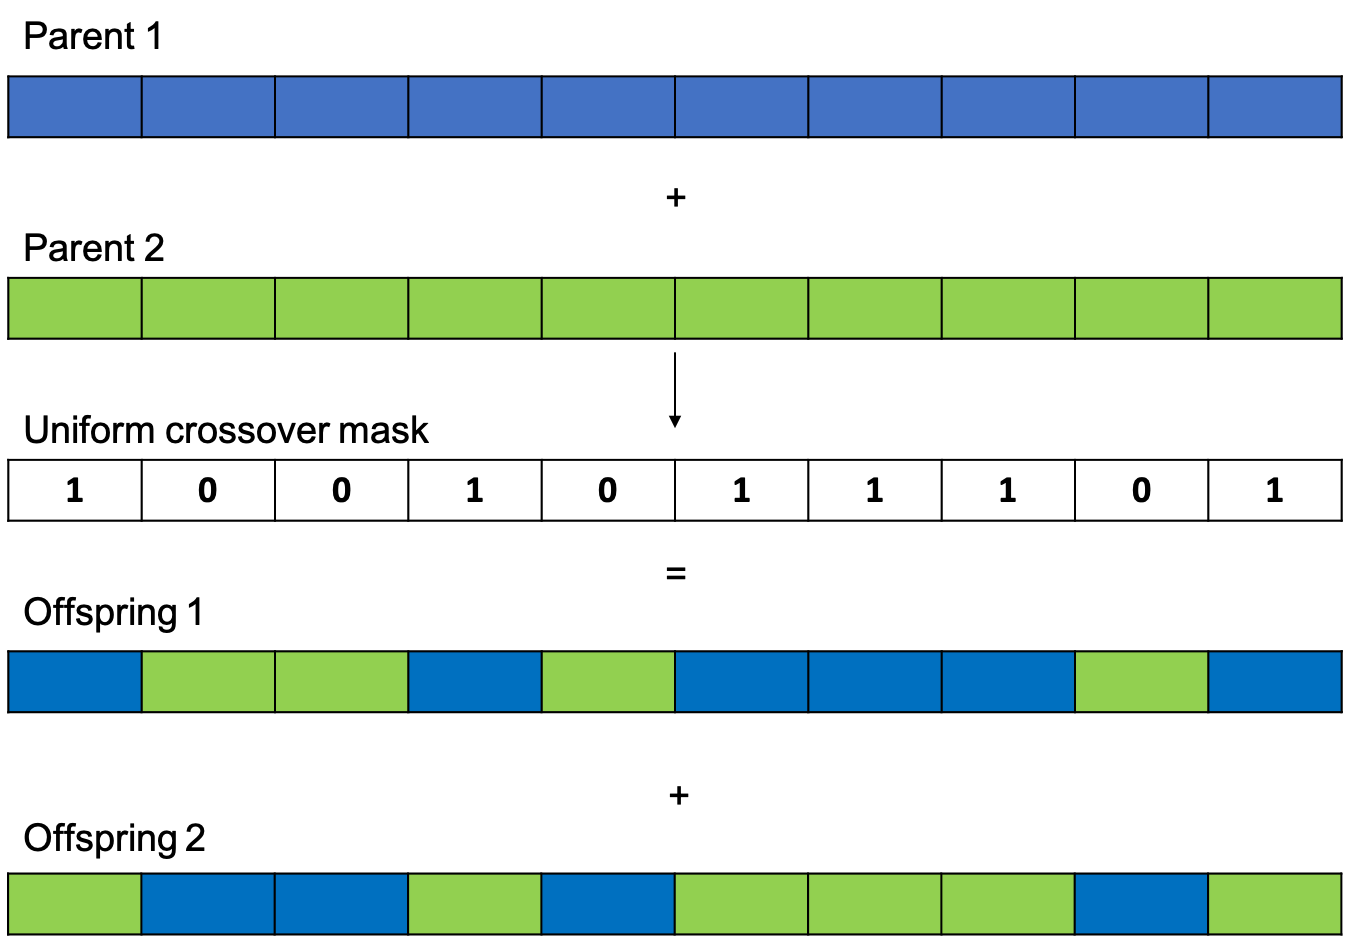
\includegraphics[width=\textwidth]{images/uniform_crossover.png}
      \caption{An illustration of the uniform crossover operator as it applies to sexual recombination, resulting in two new offspring.}
      \label{fig:heuristics:mh:ga:uniform_crossover}
\end{figure}


\begin{algorithm}[H]
      \caption{The pseudo code for the uniform crossover operator as used by \acp{GA}.}
      \label{algo:heuristics:mh:ga:uniform_crossover}
      \begin{algorithmic}
            \State Initialise the mask, $m_{j}(t) = 0 \forall j = 1, \dots, N_{x}$;
            \For{$j = 1$ to $N_{x}$}
            \If{$U(0,1) \leq p_{x}$}
            \State $m_{j}(t) = 1$;
            \EndIf
            \EndFor
            \State
      \end{algorithmic}
\end{algorithm}

In Algorithm~\ref{algo:heuristics:mh:ga:uniform_crossover} above, $p_{x}$ is the bitswapping probability.


\subsubsection{Mutation}
\label{sec:heuristics:mh:ga:mutation}

The mutation operator is applied in order to introduce new genetic material into an existing entity~\cite{ref:engelbrecht:2007}. In doing so, diversity is added into the genetic characteristics of the population. Mutation is applied at a certain mutation probability $p_{m}$ to each gene of the offspring $x_{i}(t)$ to produce mutated offspring $x'_{i}(t)$.~\citeauthor{ref:engelbrecht:2007}\cite{ref:engelbrecht:2007} mentions that the mutation probability, also referred to as the mutation rate is usually small such that $p_{m} \in [0,1]$ to ensure that good solutions are not distorted too much.

Similar to the crossover operator, mutation operators can be classified according to the representation scheme used. In the context of training
\acp{FFNN}, binary crossover operators such as the \textit{uniform} mutation operator can be used to generate a mutation mask that specifies which genes are mutated. For the purposes of this dissertation, the application of the mutation operator on $x_{ij}(t)$ results in a small update step for that gene such that $x'_{ij}(t) = x_{ij}(t) + v_{ij}(t)$. In this case, $v_{ij}(t) \sim U(-limit, limit)$ and $limit = \sqrt{\frac{6}{fanin + fanout}}$ as presented for Glorot uniform sampling in~\ref{chap:anns}. An adaptation of the uniform mutation operator is then provided in Algorithm~\ref{algo:heuristics:mh:ga:uniform_mutation} below.

\begin{algorithm}[H]
      \caption{The pseudo code for the uniform mutation operator as used by \acp{GA}.}
      \label{algo:heuristics:mh:ga:uniform_mutation}
      \begin{algorithmic}
            \For{$j = 1$ to $N_{x}$}
            \If{$U(0,1) \leq p_{m}$}
            \State Sample update step $v_{ij}(t) \sim U(-limit, limit)$
            \State $x'_{ij}(t) = x_{ij}(t) + v_{ij}(t)$;
            \EndIf
            \EndFor
            \State
      \end{algorithmic}
\end{algorithm}

An illustration of the adapted uniform mutation operator is presented in Figure~\ref{fig:heuristics:mh:ga:uniform_mutation} below.

\begin{figure}[htbp]
      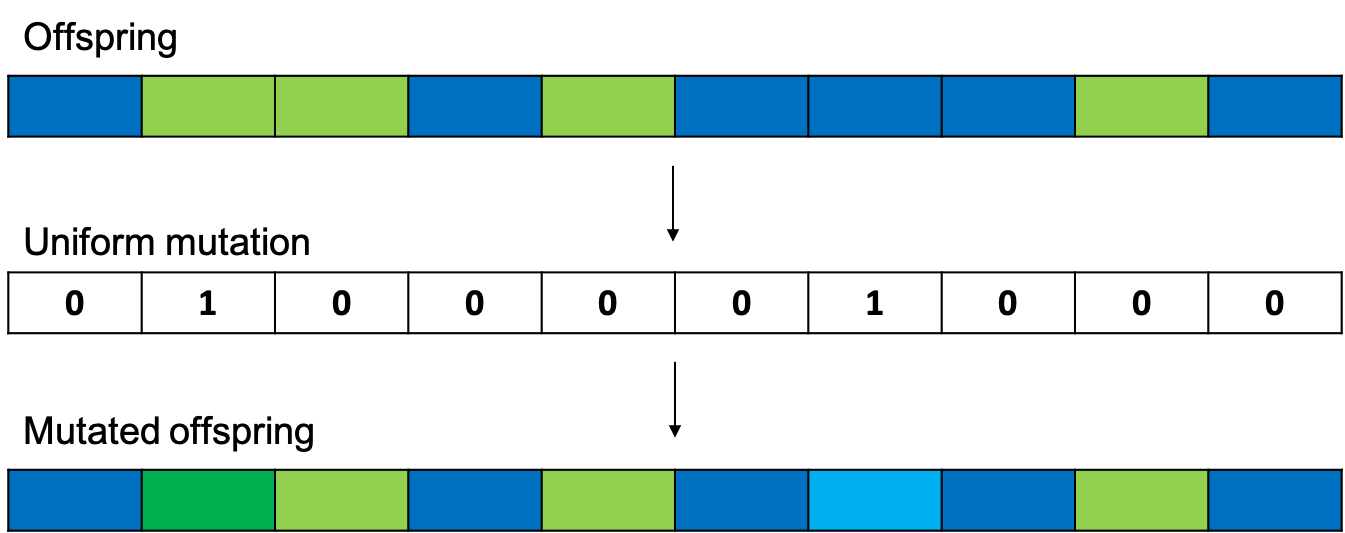
\includegraphics[width=\textwidth]{images/uniform_mutation.png}
      \caption{An illustration of the adapted uniform mutation operator as it applies to mutated offspring.}
      \label{fig:heuristics:mh:ga:uniform_mutation}
\end{figure}

\subsubsection{Selection}
\label{sec:heuristics:mh:ga:selection}

Selection is a widely used concept in all \acp{EA} and models survival of the fittest in the evolutionary context. The main idea behind the selection operator is to emphasise better solutions~\cite{ref:engelbrecht:2007}. This is done in two of the main components of \acp{EA}. These include

\begin{itemize}
      \item \textbf{Selection of the new population: } A new population of candidate solutions are is selected at the end of each generation to serve as the population for the next generation. The new population can be selected from both the parents and offspring. The selection operator is thus responsible for ensuring that good entities survive to the next generation.

      \item \textbf{Reproduction: } Offspring is created through the crossover and/or the mutation operators. In terms of crossover, good solutions should have a high probability of reproducing to ensure that offspring contain genetic material of the best entities. In terms of mutation, selection mechanisms should focus on weaker entities. By mutating weak entities, the hope is to introduce better traits, increasing their chance to survive.
\end{itemize}

\citeauthor{ref:engelbrecht:2007}\cite{ref:engelbrecht:2007} mentions that selection operators are characterised by their \textit{selective pressure}. Selective pressure is defined as the speed at which the best entity's solution will occupy the entire population by repeated application of the selection operator alone~\cite{ref:back:1994}. A selection operator with a high selective pressure rapidly decreases the diversity in the population. This could lead to premature convergence. A high selective pressure limits the exploration abilities of the population. Similar to other components and operators presented in this chapter, selection mechanisms should maintain a balance between exploration and exploitation.

Various selection mechanisms have been proposed. For the purposes of this dissertation, focus is put on the following selection mechanisms and concepts.

\begin{itemize}
      \item \textbf{Tournament Selection: } Tournament selection selects a group of $N_{ts}$ entities randomly from the population such that $N_{ts} < N_{s}$, where $N_{s}$ is the population size. The performance of the selected $N_{ts}$ entities are then compared and the best entities from this group is selected and returned by the operator. It should be mentioned that for sexual crossover of two parents, tournament selection is applied twice, first for the first parent and the again for the second parent.~\citeauthor{ref:engelbrecht:2007}\cite{ref:engelbrecht:2007} mentions that tournament selection prevents the best entities from dominating provided that $N_{ts}$ is not too large. This results in a lower selective pressure. If $N_{ts}$ is too small, the chances that bad entities will be selected increase.

      \item \textbf{Rank-based Selection: } Rank-based selection uses the rank-ordered fitness values to determine the probability of selection and not the absolute fitness value. It can therefore be said that selection is independent of actual fitness values.~\citeauthor{ref:engelbrecht:2007}\cite{ref:engelbrecht:2007} mentions that the advantage of this approach is that the best entities will not dominate the selection process. Non-deterministic linear sampling selects an entity $x_{i}(t)$ such that $i \sim U(0, U(0, N_{s} - 1))$. Importantly, in the context of a minimisation problem, entities are first sorted in decreasing order of fitness value, assuming that the best heuristic is then contained at index 0, while the worst entity is contained at index $N_{s} - 1$.

      \item \textbf{Elitism: } Elitism refers to the process of ensuring that the best entities from the current population survive to the next generation. The best entities are simply passed on to the next generation without mutation. The more entities that survive to the next generation, the lower the diversity of the new population. It is later shown in~\ref{chap:bhh} that the proposed \ac{BHH} can incorporate a form of elitism in its credit assignment strategy.
\end{itemize}


\subsubsection{Control Parameters}
\label{sec:heuristics:mh:ga:control_parameters}

Throughout this section a number of control parameters have been provided that affect the performance of the \acs{GA}. These include the population size $N$, the crossover rate $p_{c}$ and the mutation rate $p_{m}$.~\citeauthor{ref:engelbrecht:2007}\cite{ref:engelbrecht:2007} mentions that these values are usually kept static. However, it is widely accepted that these parameters have a significant impact on the performance of the \acs{GA}.  Finding optimal values for $p_{c}$ and  $p_{m}$ empirically can be a time consuming process. As such, dynamic parameter values can be introduced, however, this is beyond the scope of this dissertation.


\section{Summary}
\label{sec:heuristics:summary}

This chapter provided the reader with detailed background information on different heuristics that have been shown to be able to train \acp{FFNN}. Two main groups of heuristics where discussed. These include gradient-based heuristics and \aclp{MH}. For each of these groups a number of different variants have been discussed. A total of ten different heuristics have been introduced and where possible, their advantages, disadvantages and characteristics have been discussed.

The next chapter aims to build on the foundations provided in this chapter by putting focus on \acp{HH}. It is shown that \acp{MH} implement a heuristic pool of lower-level heuristics such as those presented in this chapter.










